\chapter{Visualization Tools}
\label{cpt:tools}

The main contribution of this project is automatic methods for visualizing how a webcam scene varies and for understanding the most important variations.  In most natural scenes, we notice changes in lighting, weather, and camera conditions which fail to describe the typical behavior of a scene.  The goal of these tools is to learn these variations and to point out changes independent of them.  PCA is a commonly used tool, and
captures a linear model of consistent image variations.  By analyzing the results of certain PCA trials, we can obtain important and interesting information.

\section{PCA Input}

A naive algorithm to learn about scenes is to take the PCA of the entire webcam scene.  Modifying our input, however, can produce better results.

\subsection{Temporal Narrowing}

The AMOS Dataset consists mostly of outdoor scenes.  These outdoor scenes vary significantly over the course of a day, going from night to day and back.  The change in lighting dominates all other changes across the scene, and causes many images to be dark and noisy.  Instead of wasting PCA basis vectors on learning this change, we can limit our input to daytime images which we expect to be well-lit.  This strategy is used for all scenes.

\subsection{Sky Mask}
In many outdoor scenes, even when narrowed to a particular time of day, the most difficult image variation to characterize is the sky.  PCA has a difficult time learning changes in sunlight, clouds,
and other sky-based variation.  The variance in the sky dominates the PCA reconstruction, causing the basis vectors to focus less on more important variation, as shown in Figure \ref{fig:skyMaskFig}.

\begin{figure}[t]
	\centering
		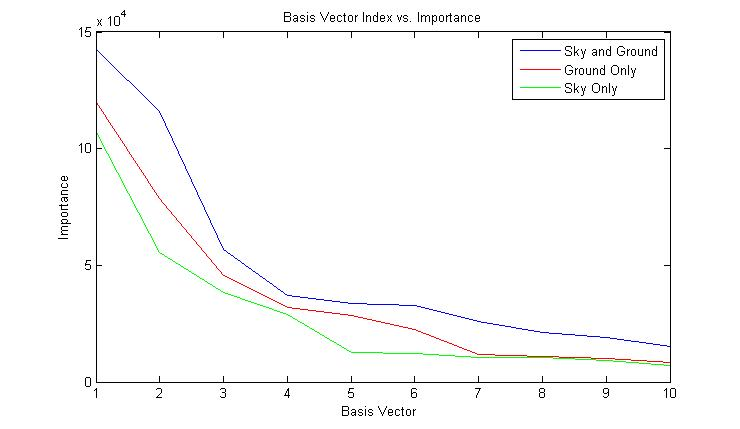
\includegraphics[width=.7\textwidth]{figures/skyMaskFig.jpg}
	
		\caption[Singular values of scenes with and without the sky.]{The plot shows the singular value, or importance, or each of the ten basis vectors for PCA on a scene with both the sky and ground, with the ground only, and with the sky only.  Since the latter two's singular values do not at up to the former's, we can conclude that looking at the ground only captures more information about the ground than looking at both concurrently.}
		
	\label{fig:skyMaskFig}
\end{figure}

Fortunately, it is fairly easy to learn which regions of an image should be labeled as sky.  A side effect of the rising and setting of the sun is that the first principal component of most scenes - looking at all images, not just daytime images - is the sky, as shown in \ref{fig:2skyPCA}.  By thresholding the values of this vector, we can effectively segment the sky from the rest of the image, as shown in \ref{fig:2skyMask}.

This simple mask allows PCA to focus on more interesting changes in the image, and most of the results that follow use a simple mask to ignore the sky regions of the images.  By setting all pixels values in the sky to 0, we can effectively remove this difficulty.


		
\begin{figure}[ht]
	\centering
	\subfigure[]{
		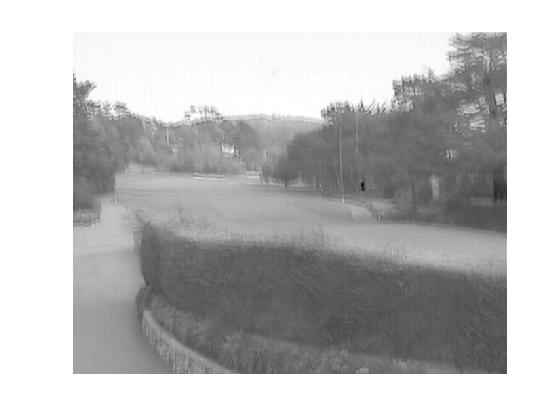
\includegraphics[width=0.45\textwidth]{figures/2skyPCA.jpg}
	\label{fig:2skyPCA}
	}
	\subfigure[]{
		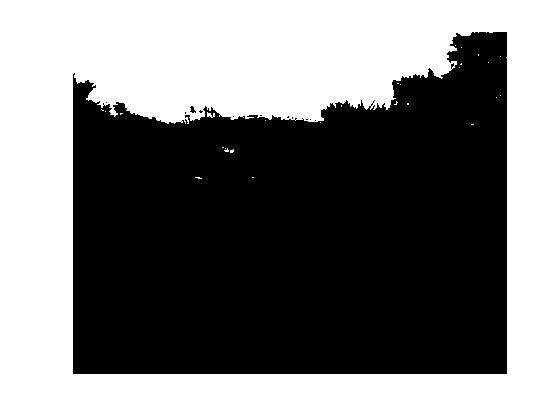
\includegraphics[width=0.45\textwidth]{figures/2skyMask.jpg}
	\label{fig:2skyMask}
	}
		\caption[Learning a sky mask for a webcam scene.]{Figure \ref{fig:2skyPCA} shows the first PCA component of a webcam scene.  By adding or subtracting this component, we control how dark or how light the sky is. Figure \ref{fig:2skyMask} shows that a simple thresholding of this image effectively segments the sky from the rest of the image.}\end{figure}
		
\subsection{Gradient Image}

\begin{figure}[htp]
	\centering
	\subfigure[]{
		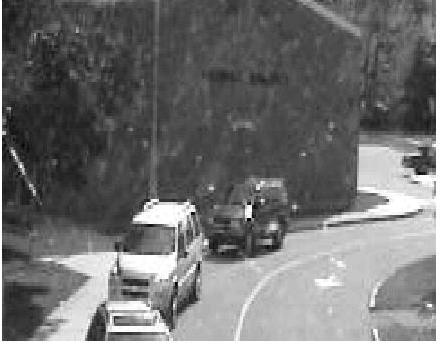
\includegraphics[width=0.45\textwidth]{figures/194cars.jpg}
	\label{fig:carsNoGradient}
	}
	\subfigure[]{
		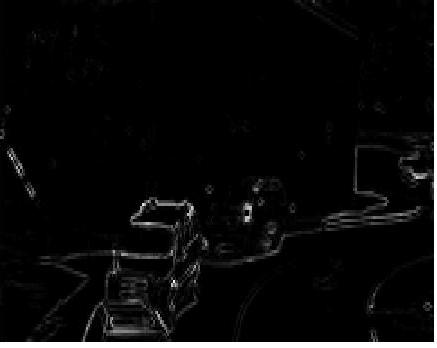
\includegraphics[width=0.45\textwidth]{figures/194carsGradient.jpg}
	\label{fig:carsGradient}
	}
		\caption[Highlighting object edges with gradient magnitude images.]{Figure \ref{fig:carsNoGradient} shows a grayscale webcam image. Figure \ref{fig:carsGradient} shows its gradient magnitude image.  Notice the noise is mostly removed and the edges of the vehicles and building are highlighted.}
\end{figure}

The gradient magnitude image highlights edges in an image, as they are image locations where pixel values differ greatly from their neighbors.  By performing PCA on the gradient magnitude images, we tend to ignore the potentially noisy surfaces of objects, and instead focus on the locations of the objects.  Figure \ref{fig:carsNoGradient} and Figure\ref{fig:carsGradient} show the edges of an interesting webcam image highlighted in a gradient magnitude image.


The x and y derivatives of an image are approximated as $I_x(x,y) = I(x,y)-I(x-1,y)$ and $I_y(x,y) = I(x,y)-I(x,y-1)$ where the function $I(x,y)$ describes the intensities of an image's pixels.  Once we have calculated the derivative images, we define the gradient magnitude of an image to be $G(x,y) = \sqrt{I_x(x,y)^2 + I_y(x,y)^2}$.

In practice, taking PCA of the gradient magnitude image does not add much to our results, so we bypassed this step in our work.


\pagebreak{}
\section{Visualizations}

In this section, we present several tools to visualize the webcam scene once we have evaluated the PCA error.

\begin{figure}[p]
	\centering
	\subfigure[]{
		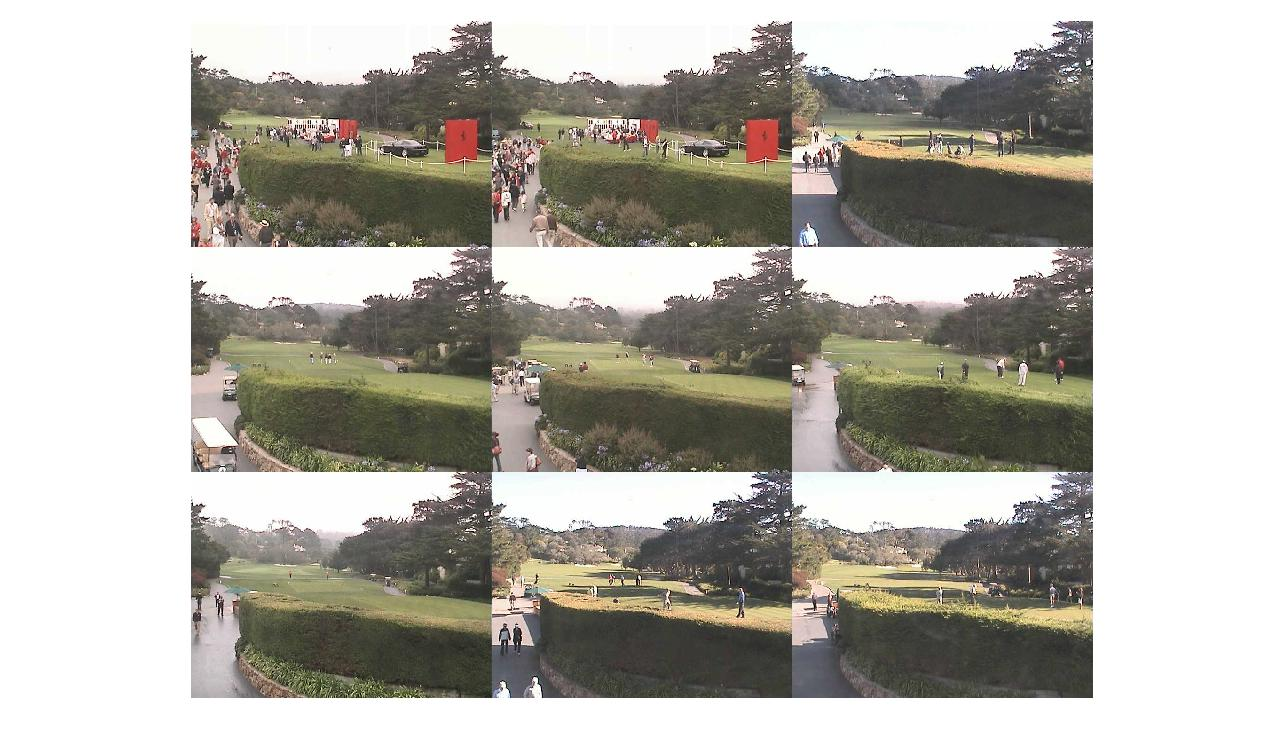
\includegraphics[width=.8\textwidth]{figures/golfMontageNaive.jpg}
	\label{fig:golfMontageNaive}
	}
	\subfigure[]{
		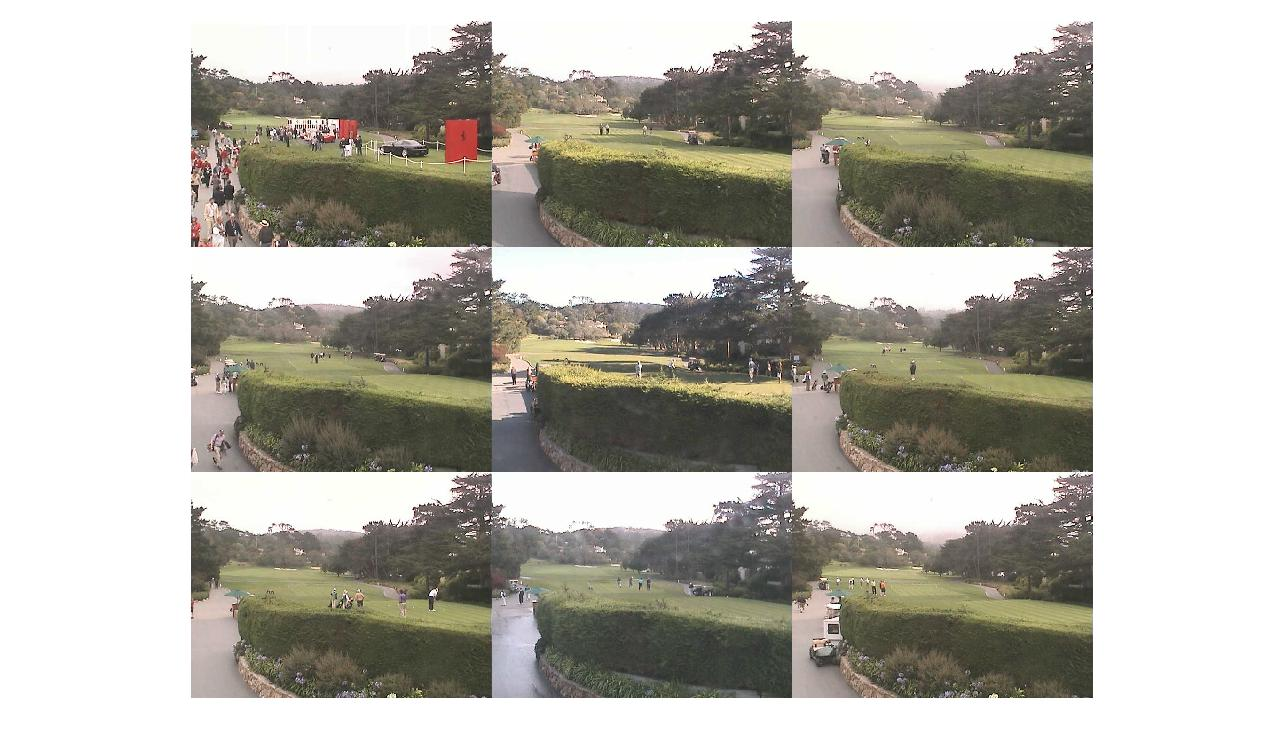
\includegraphics[width=.8\textwidth]{figures/golfMontageSmart.jpg}
	\label{fig:golfMontageSmart}
	}
		\caption[Image montage techniques.]{Figure \ref{fig:golfMontageNaive} shows a montage of interesting images from a golf course scene. Figure \ref{fig:golfMontageSmart} shows a montage of interesting images of the same scene using the Well-Separated Set technique.}
\end{figure}

\subsection{Image Montage}

A simple way to visualize a webcam scene is to view a montage of several images from that scene.  We can easily sort the images along some dimension, and then show the $n$ images with the highest values in that dimension.  Figure \ref{fig:golfMontageNaive} Is an example montage of several interesting images from a golf course scene.

\subsection{Well-Separated Set Montage}

In several of these montages, we notice that many of the most unusual images are similar to each other.  This presents the problem of finding unusual images that are different from the images we have already chosen.

A simple but effective algorithm for this problem uses the L2 norm in image space.  If we consider an image as a vector of pixel intensities, such as $v = \{v_1, ..., v_m\}$, the L2 norm of two images $v$ and $u$ is $$L2\_norm(v,u) = \sqrt{\sum_{i=1}^m{(v_i-u_i)^2}}$$  Given a large set of unusual images $\{x_1, ..., x_n\}$, we compute a distance matrix $D$ where $D_{i,j} = L2\_norm(x_i, x_j).$  Now we iteratively find unusual images by choosing the image that has the largest distance from all of the images we have chosen so far.  Specifically, for each remaining image calculate its distance to our set of exemplars, and choose the image whose distance is the smallest.  We define the distance of an image $x_0$ to a set of exemplars $\{x_1, ..., x_n\}$ as $$d = \min_i(D(x_0, x_i))$$Then we can choose the image that has the highest value of this distance.  In this way, on each iteration, we pick the image that is least likely to be similar to an image we have already selected.  Figure \ref{fig:golfMontageSmart} shows how this technique omits similar images.

\subsection{Two-dimensional Explorer}

\begin{figure}[h]
	\centering
		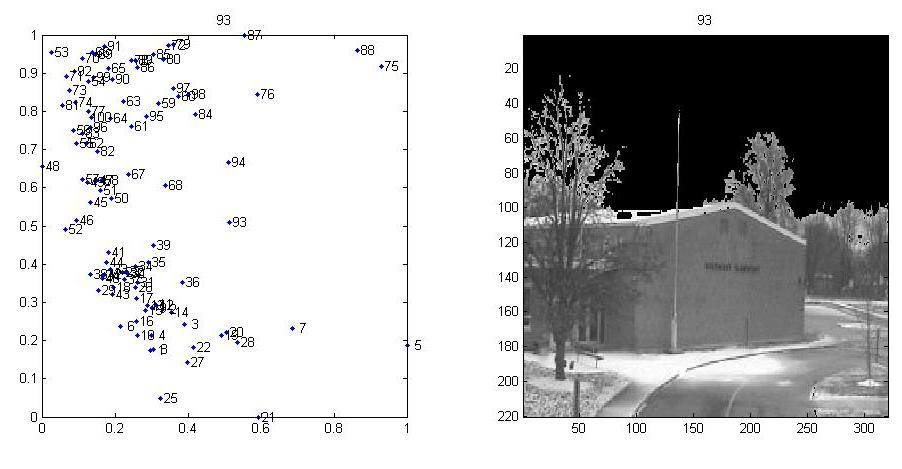
\includegraphics[width=1\textwidth]{figures/2dGui.jpg}
	
		\caption[Exploring 2D image space using a simple GUI.]{This figure shows a webcam scene displayed using the 2D GUI.}	
		
	\label{fig:2dGui}	
\end{figure}

Using a simple GUI, we can explore a webcam scene in two dimensions.  The GUI, shown in \ref{fig:2dGui}, displays a a plot of image scores for two different criteria, and displays the image corresponding to the highlighted data point.  Using this GUI, it is possible to see which evaluations are related and which are not, and makes it easier to learn how the evaluations appear in image space.


\section{Characteristics of Image Reconstructions and Residuals}

Once webcam scenes are projected onto a PCA basis, there are many different ways to analyze the results.  In this section, we will present several different methods for evaluating this appearance model of a scene.

\subsection{PCA Basis Coefficient Vector Magnitude}

\begin{figure}
	\centering
	\subfigure[]{
		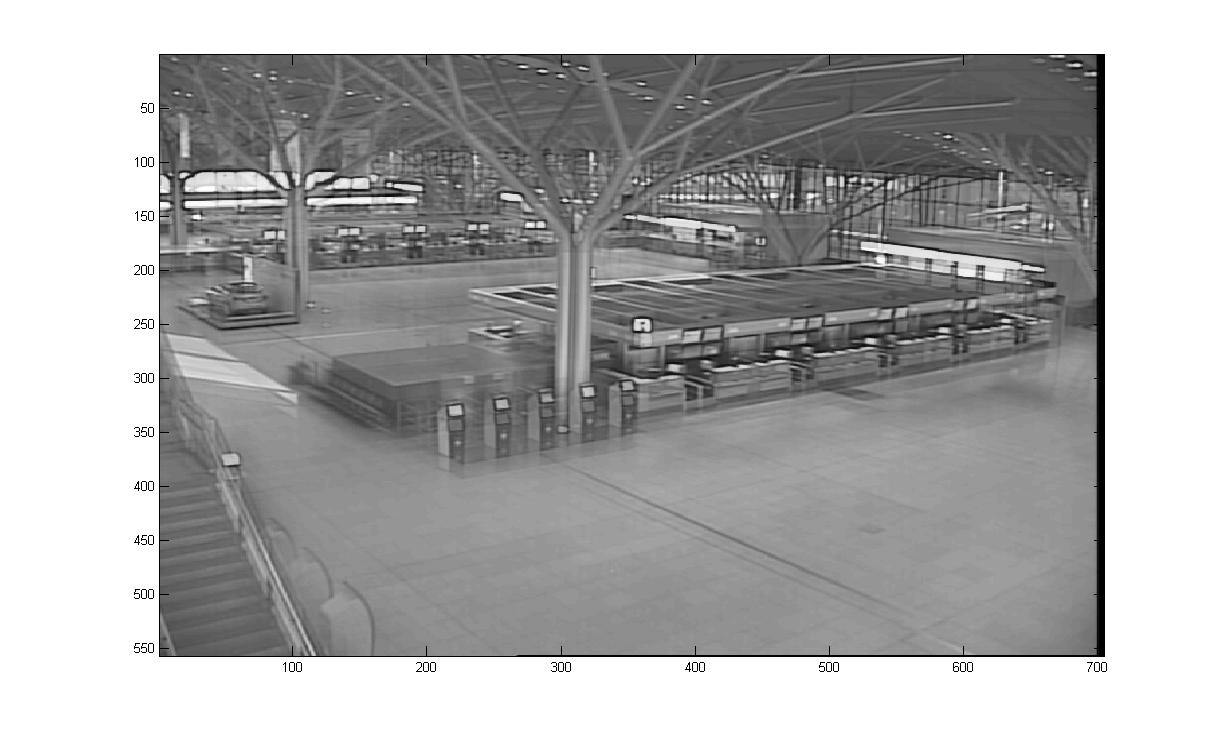
\includegraphics[width=.7\textwidth]{figures/vectorMagnitudeMean.jpg}
	\label{fig:vectorMagnitudeMean}
	}
	\subfigure[]{
		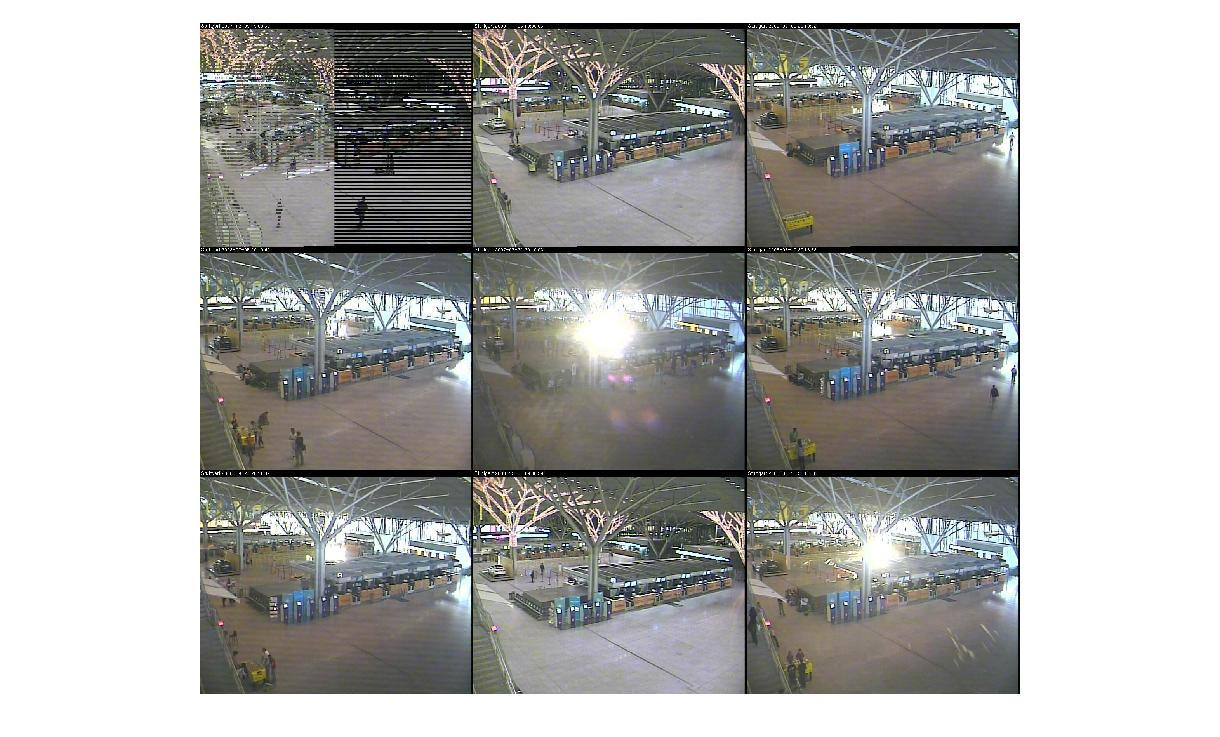
\includegraphics[width=.7\textwidth]{figures/vectorMagnitudeMontage.jpg}
	\label{fig:vectorMagnitudeMontage}
	}
		\caption[PCA Basis Coefficient Vector Magnitude.]{Figure \ref{fig:vectorMagnitudeMean} shows the mean image of an airport scene. Figure \ref{fig:vectorMagnitudeMontage} shows several images found using this technique that are far from the mean.}
\end{figure}

For each image in a scene, PCA gives a vector of coefficients that correspond to the best linear combination of basis images to reconstruct that image.  From this vector, we can assign each image a score equal to the magnitude of this vector.  For a vector $v = (v_0, v_1, ..., v_n)$, the vector magnitude is $$||v||=\sqrt{\sum_{i=0}^nv_i^2}$$This effectively gives us a measure for how far from the mean image in our basis space each image is.  Figure \ref{fig:vectorMagnitudeMean} shows the mean image of a webcam scene and Figure \ref{fig:vectorMagnitudeMontage} shows several images from that webcam scene that are especially far from the mean.  Evaluating and montaging images a scene in this way is an effective strategy for finding interesting images, but gives no semantics as to how the images are interesting.

\subsection{Residual Error}

Given an image and a PCA basis, we can project the image onto the basis and see how well we this reconstructs the image by analyzing the residual image, as shown in Figure \ref{fig:residualReconstruction}.

\begin{figure}[h!]
	\centering
		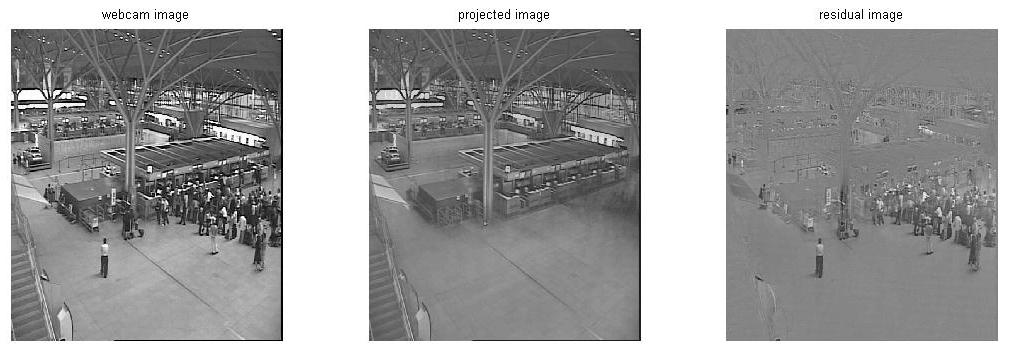
\includegraphics[width=1\textwidth]{figures/residualReconstruction.jpg}
	
		\caption[The reconstruction and residual of an image.]{This figure shows a webcam scene image, the reconstruction of that image from a PCA basis, and the residual image.  Notice how the residual image contains most of the foreground objects.}
		
	\label{fig:residualReconstruction}
\end{figure}

\begin{figure}
	\centering
		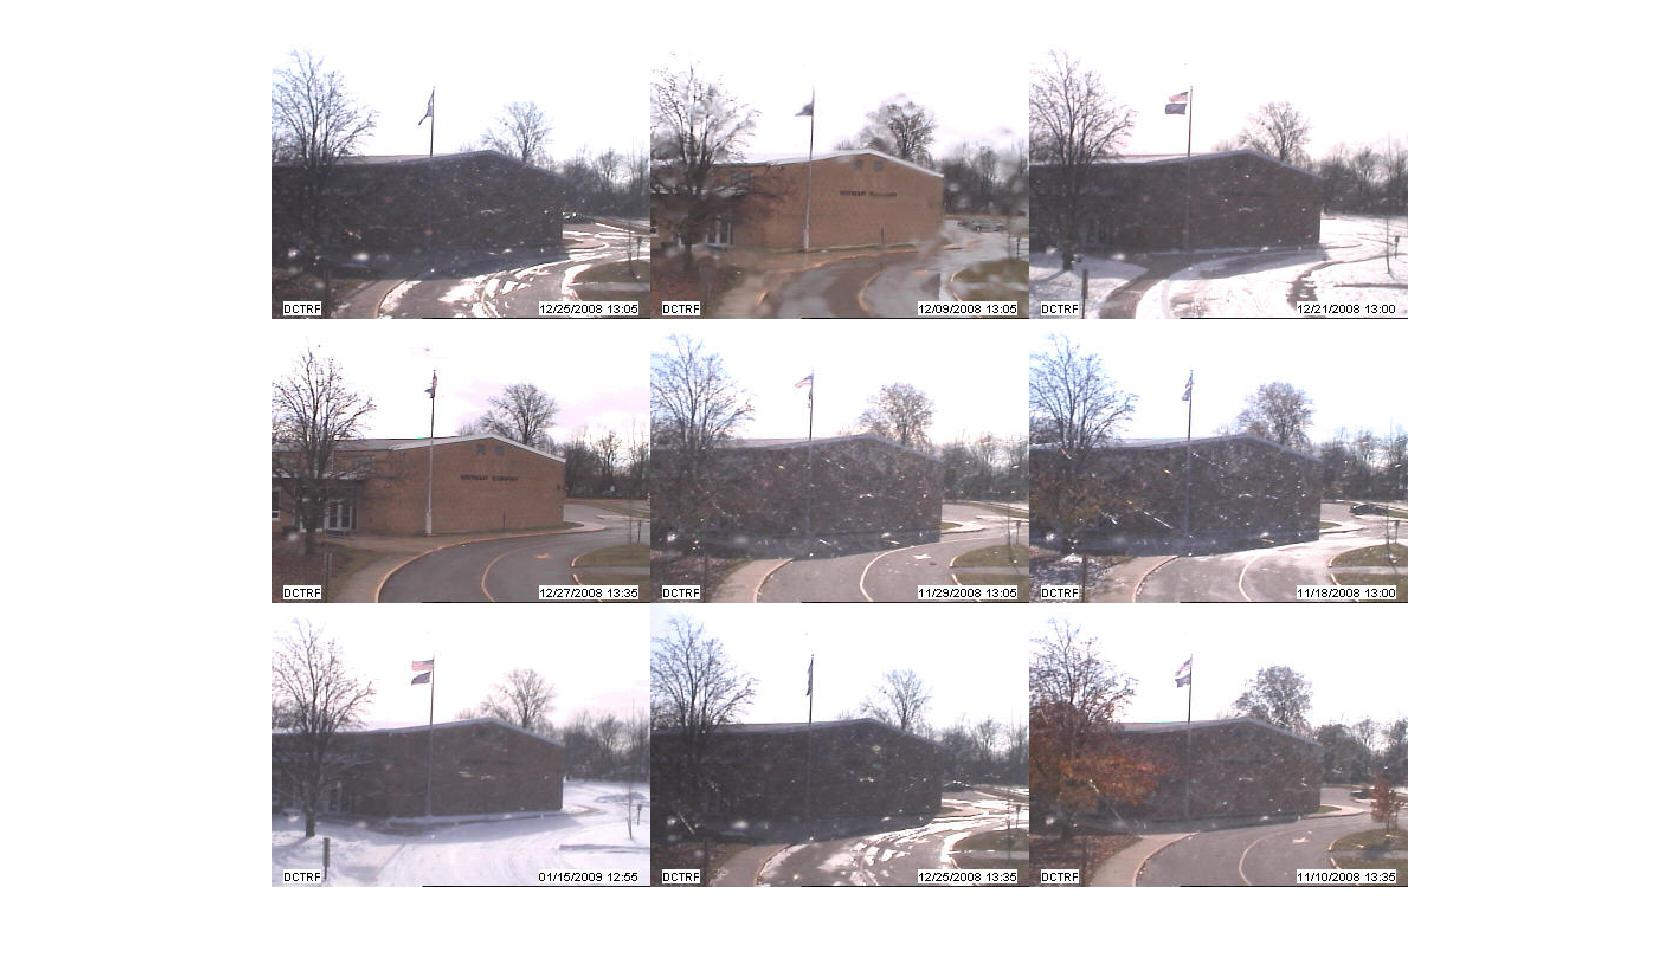
\includegraphics[width=1\textwidth]{figures/residualSSDmontage.jpg}
	
	
		\caption[Sum Squared Residual Montage.]{This figure shows a the most interesting images from a golf course scene sorted by the sum of the squared residual values.}
		\label{fig:residualSSDmontage}
\end{figure}

If we sort evaluate our images based on the sum of the squared residual values of each pixel, we get a good measure for how much variation is not captured by PCA, as shown in Figure \ref{fig:residualSSDmontage}.  Whereas the PCA coefficient vector magnitude evaluation gives images that are different from the mean image, this evaluation captures more of the interesting variation that we are looking for.


\subsection{Variance Model}

We can estimate the variance image of a webcam scene as the average of the square of each residual image.  This image gives a good summary as to where most activity occurs in a webcam scene.  Several examples are shown in Figure \ref{fig:severalVarianceImages}.

\begin{figure}
	\centering
		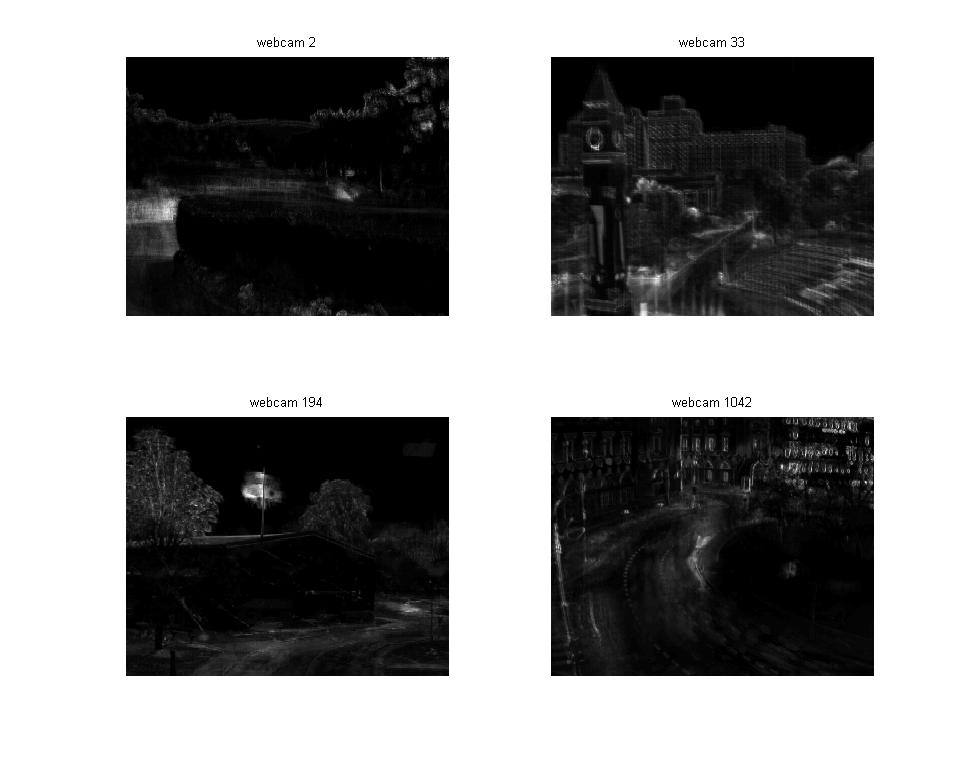
\includegraphics[width=1\textwidth]{figures/severalVarianceImages.jpg}
	
	
		\caption[Several variance images.]{This figure shows estimated variance images from several webcam scenes.}
		\label{fig:severalVarianceImages}
\end{figure}

One we have this variance image, we can attempt to isolate independent pixels in a z-score image.  We define our z-score image as $$Z(x,y) = \frac{R(x,y)} { V(x,y)}$$ where $R(x,y)$ is the residual value of the pixel and $V(x,y)$ is the variance value of the pixel.  By summing the per pixel z-score for an particular image, we can infer how atypical the residual of that image is.  Figure \ref{fig:residualZScoreMontage} shows several images that contain atypical objects.  Such a tool can be used to quickly highlight unusual behavior in a scene, such as unusual shots on a golf course or security breaches in a bank scene.

\begin{figure}
	\centering
		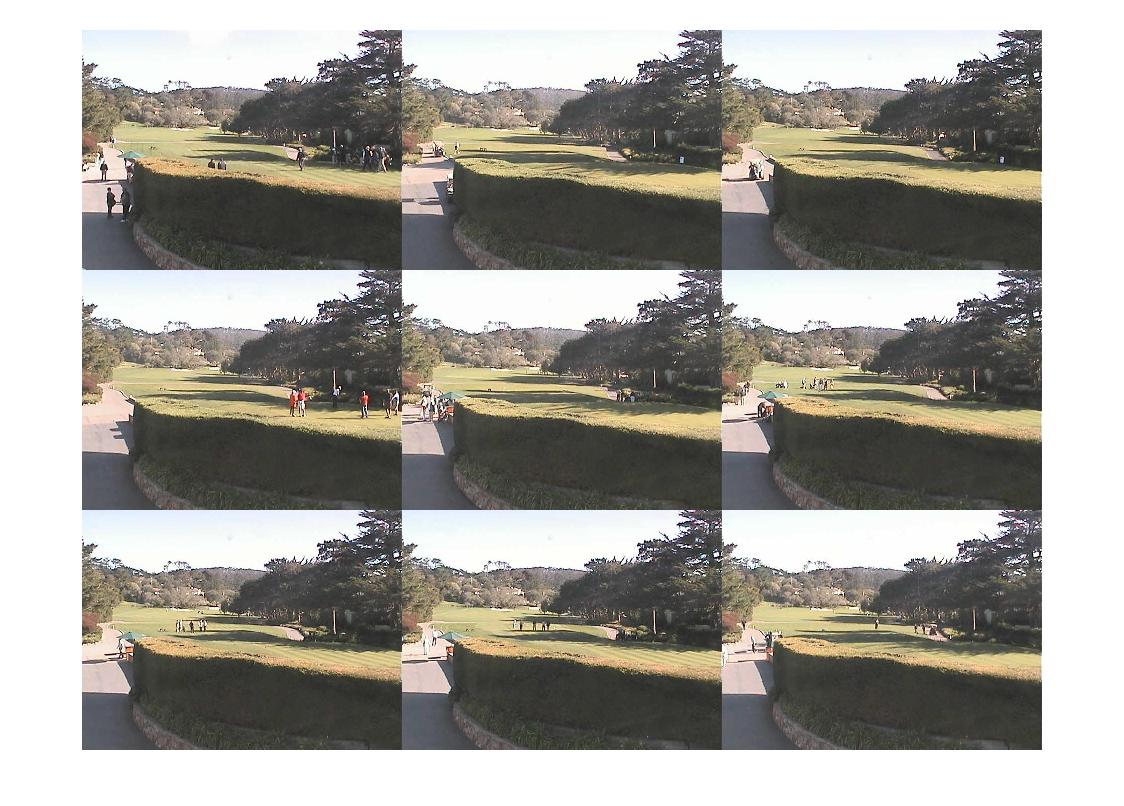
\includegraphics[width=1\textwidth]{figures/residualZScoreMontage.jpg}
	
	
		\caption[Z-Score Montage.]{Figure \ref{fig:residualZScoreMontage} shows several images from the same scene as \ref{fig:residualSSDmontage}, but sorted by the sum of the Z-Score values.  The objects in these images are in more unlikely positions as those in the residual sum squared error montage.}
		\label{fig:residualZScoreMontage}
\end{figure}





\subsection{Statistical Distribution of Residual Images}



\begin{figure}[htp]
	\centering
	\subfigure[]{
		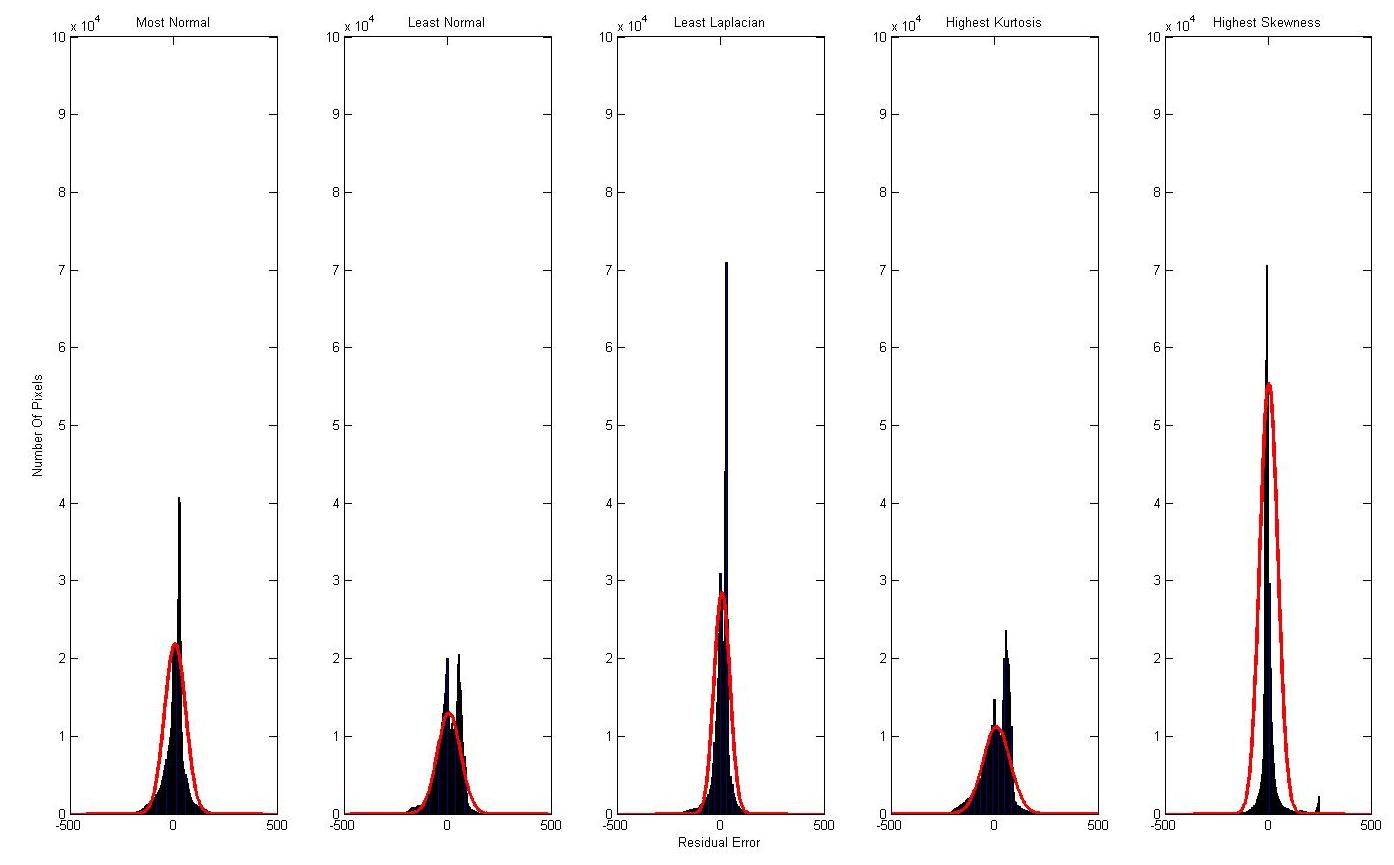
\includegraphics[width=.6\textwidth]{figures/severalHists2.jpg}
	\label{fig:severalHistsPlot}
	}
	
	\subfigure[]{
		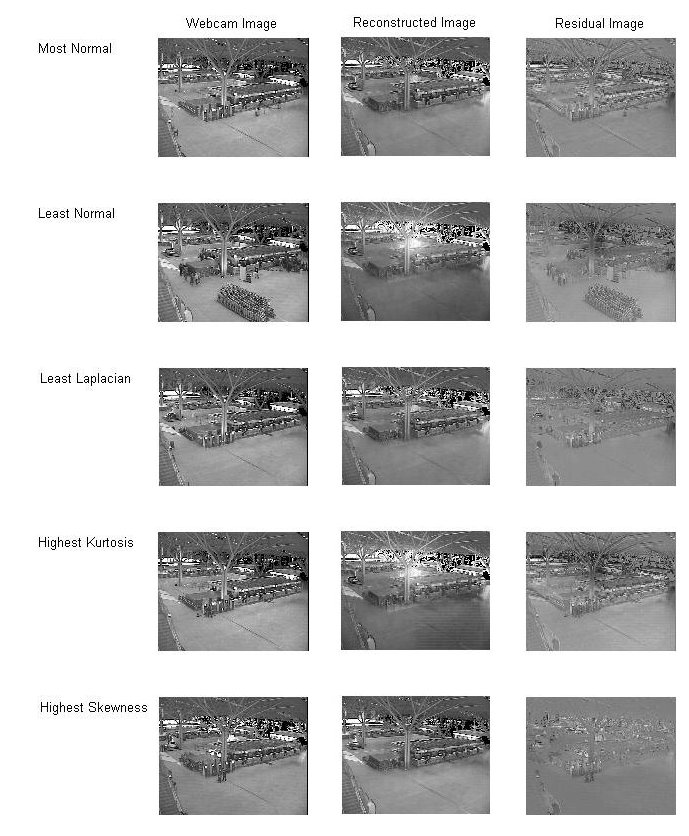
\includegraphics[width=.6\textwidth]{figures/severalHistsReconstruction.jpg}
	\label{fig:severalHistsReconstruction}
	}
	
		\caption[Several residual image histograms.]{Figure \ref{fig:severalHists} shows several residual image histograms and the the best approximation of a normal distribution fitting the data.  Figure \ref{fig:severalHistsReconstruction} shows the image corresponding to each histogram and the corresponding reconstructed images and residual images.}
		\label{fig:severalHists}
\end{figure}

We can also try to learn about an image reconstruction by treating its residual image as samples from an 
underlying probability density function.  If image deviations are due mostly to noise, we predict that these deviations will be normally distributed, but as shown in Figure \ref{fig:severalHists}, this is not always the case.  We have found that these distributions vary in the same way as webcam scenes, and analyzing them in the right way tells an interesting story.



\begin{figure}
	\centering
	\subfigure[]{
		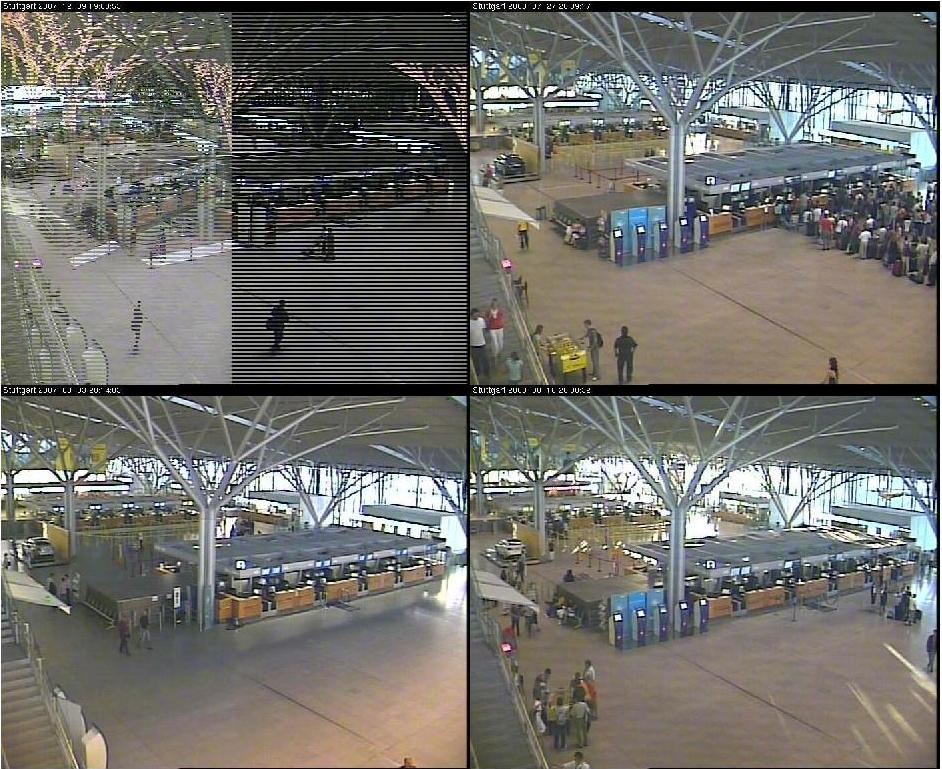
\includegraphics[width=.6\textwidth]{figures/leastNormal.jpg}
	\label{fig:leastNormal}
	}
	
	\subfigure[]{
		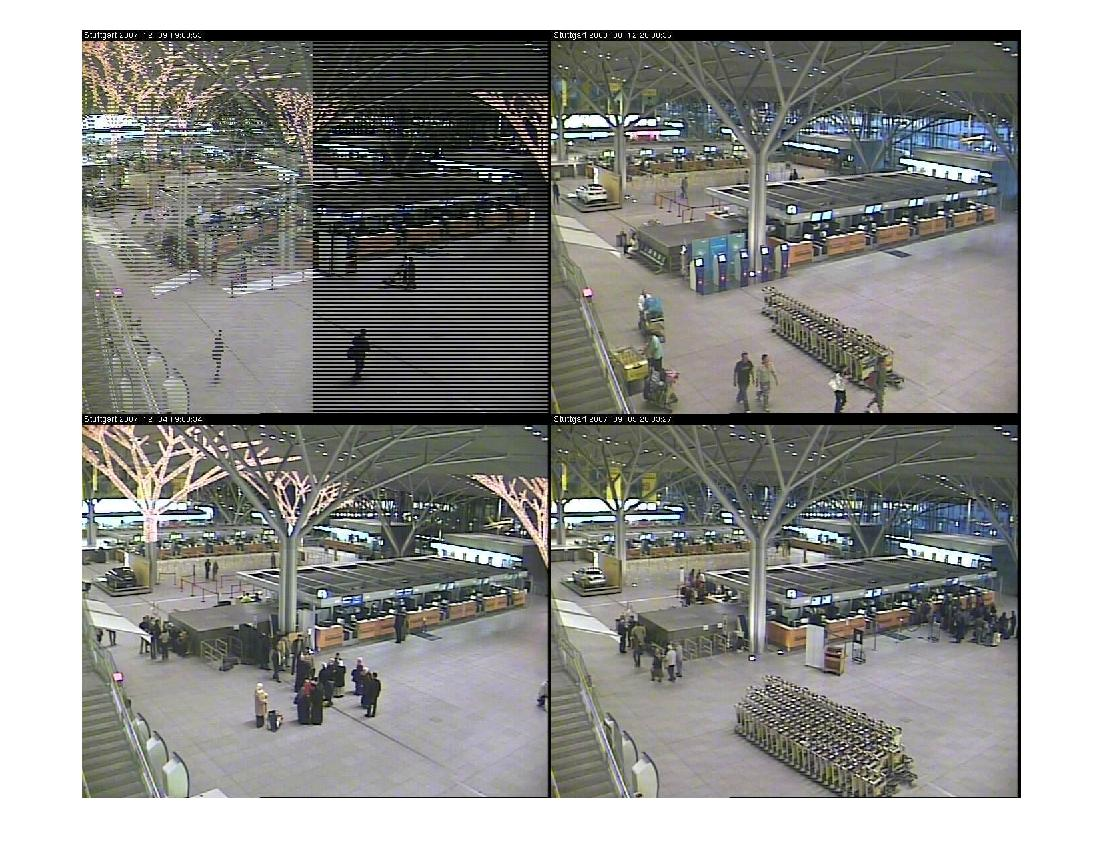
\includegraphics[width=.6\textwidth]{figures/leastLaplacian.jpg}
	\label{fig:leastLaplacian}
	}
	
			\caption[Least Gaussian and Least Laplacian Image Montages.]{Figure \ref{fig:leastNormal} shows a montage of interesting images from an airport scene that were labeled very non-Guassian. Figure \ref{fig:leastLaplacian} shows a montage of interesting images from an airport scene that were labeled very non-Laplacian.  Notice that the least Laplacian images contain foreground objects than do the least Guassian images.}
\end{figure}



\begin{enumerate}
\item{\textbf{Gaussian Likelihood}}

A simple strategy is to treat each residual image pixel as a sample from a Gaussian distribution.  We can easily estimate the mean and variance of this PDF and then, for each residual value, use the Gaussian distribution equation 

$$f(x|\mu,\sigma)=\frac{1}{\sigma\sqrt{2\pi}}e^{\frac{(x-\mu)^2}{2\sigma^2}}$$

to evaluate the overall likeliness that the residual image was sampled from the estimated Gaussian distribution.  

Figure \ref{fig:leastNormal} shows a Well-Separated Set Montage of images that were not likely Gaussian.  These images capture some interesting variation, but also some variation in lighting and camera artifacts.

\item{\textbf{Laplacian Likelihood}}

Many of the residual images have a majority of pixels that are very close zero.  This causes the histogram to look very similar to the Laplacian distribution.  We can estimate the Laplacian likeliness in the same way as for Gaussian distribution, but using the Laplacian distribution definition

$$f(x|\mu,\beta)=\frac{1}{2\beta}e^{\frac{-|x-\mu|}{\beta}}$$

Figure \ref{fig:leastLaplacian} shows a Well-Separated Set Montage of images that were not likely Laplacian.  These images tend to capture more interesting variation than those in Figure \ref{fig:leastNormal}.

\item{\textbf{Kurtosis}}

The kurtosis of a real-valued random variable is a measure of its peakedness.  Larger values of kurtosis means more variance is due to less frequent extreme deviations rather than frequent less extreme deviations.  It is defined as $$\gamma_2=\frac{\mu_4}{\sigma^4}$$ where $\mu_4$ is the fourth moment about the mean and $\sigma^4$ is the estimated standard deviation to the fourth power.  For a function $f(x)$, the $k^{th}$ moment about the mean is defined as 

$$\mu_k = \int_{-\infty}^{\infty}{(x-\mu)^kf(x)dx}$$

Evaluating images based on the kurtosis of their residual images tend to give results that mirror the images sorted by sum of the squared residual values.   

\item{\textbf{Skewness}}

The skewness of a random variable is a measure of asymmetry.  Higher skewness values mean deviations on one side of the mean do not have corresponding deviations on the other side.  It is defined as $$\gamma_1=\frac{\mu_3}{\sigma^3}$$ where $\mu_3$ is the third moment about the mean and $\sigma^3$ is the cube of the standard deviation.

Evaluating images based on skewness does not give positive results.  The is possibly the result of the fact that small objects on either side of the mean that would add to the asymmetry of the distribution are dominated by the noise over the rest of the image.


\end{enumerate}


